\chapter{Literature Study}
\label{chap:literature}

\npar The mobile industry is without a doubt one of the most vibrant industries at the moment. Not only because mobile device sales are growing rapidly but also because of the highly competitive nature of this market. This has led to fragmentation. 

\npar This chapter will sketch the landscape of mobile devices, explain the problem of fragmentation and a number of suggested solutions to cope with this problem.

\section{The mobile device landscape}

\npar In the last couple of years, smartphone sales have gone up quickly. Smartphones are becoming ubiquitous and in some regions, like the United States, smartphone penetration has already reached more than 50\% \cite{Nielsen:2012}. According to quarterly studies by Gartner, smartphone penetration remained stable before the iPhone 3G and Android came along (see \fref{fig:smartphone_sales}).

\begin{figure}[h!]
    \begin{center}
        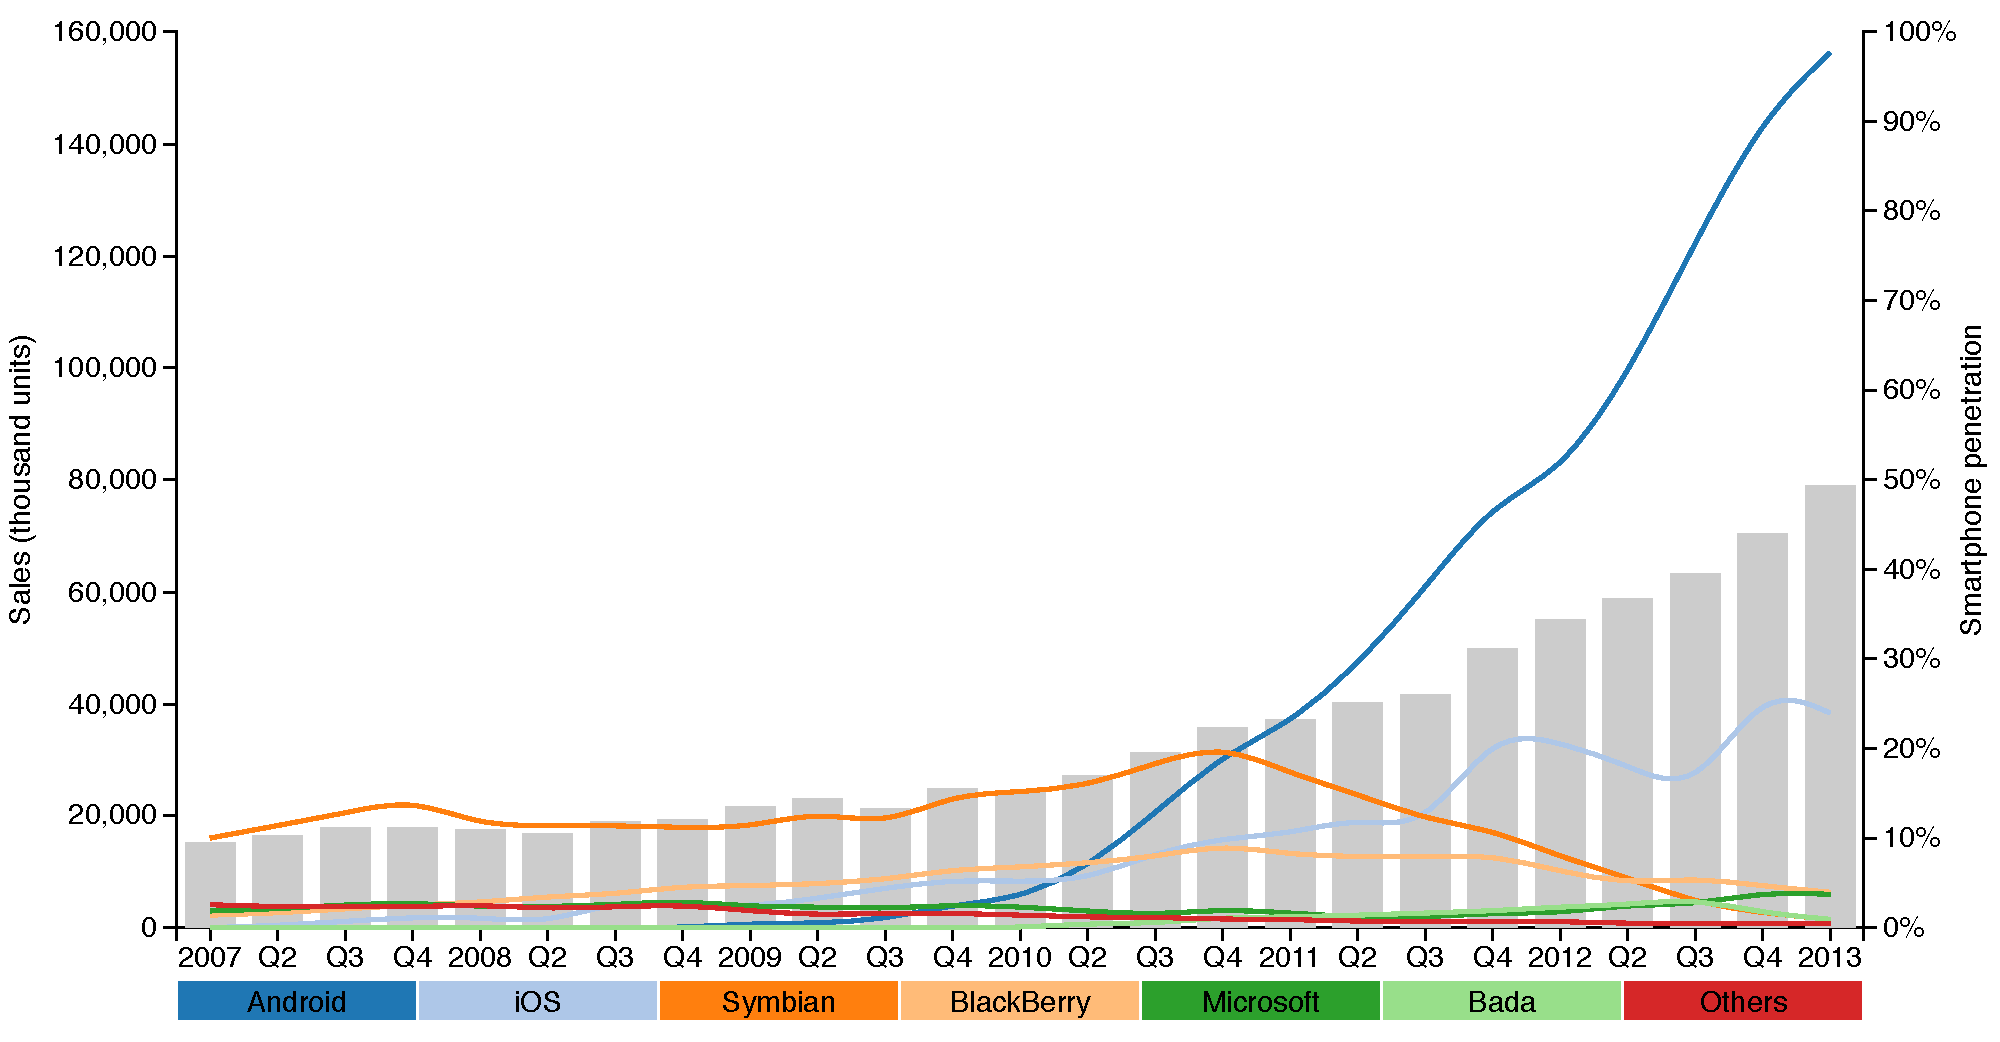
\includegraphics[width=\textwidth]{figs/smartphone_sales.pdf}
        	\caption{
        	    	Growth of worldwide smartphone sales and smartphone penetration. Source: Gartner \citep{Gartner:08Q2,Gartner:08Q3,Gartner:08Q4,Gartner:10Q1,Gartner:10Q2,Gartner:10Q3,Gartner:10Q4,Gartner:11Q1,Gartner:11Q2,Gartner:11Q3,Gartner:11Q4,Gartner:12Q1,Gartner:12Q2}
        	}
        	\label{fig:smartphone_sales}
    \end{center}
\end{figure}

\begin{figure}[h!]
    \begin{center}
        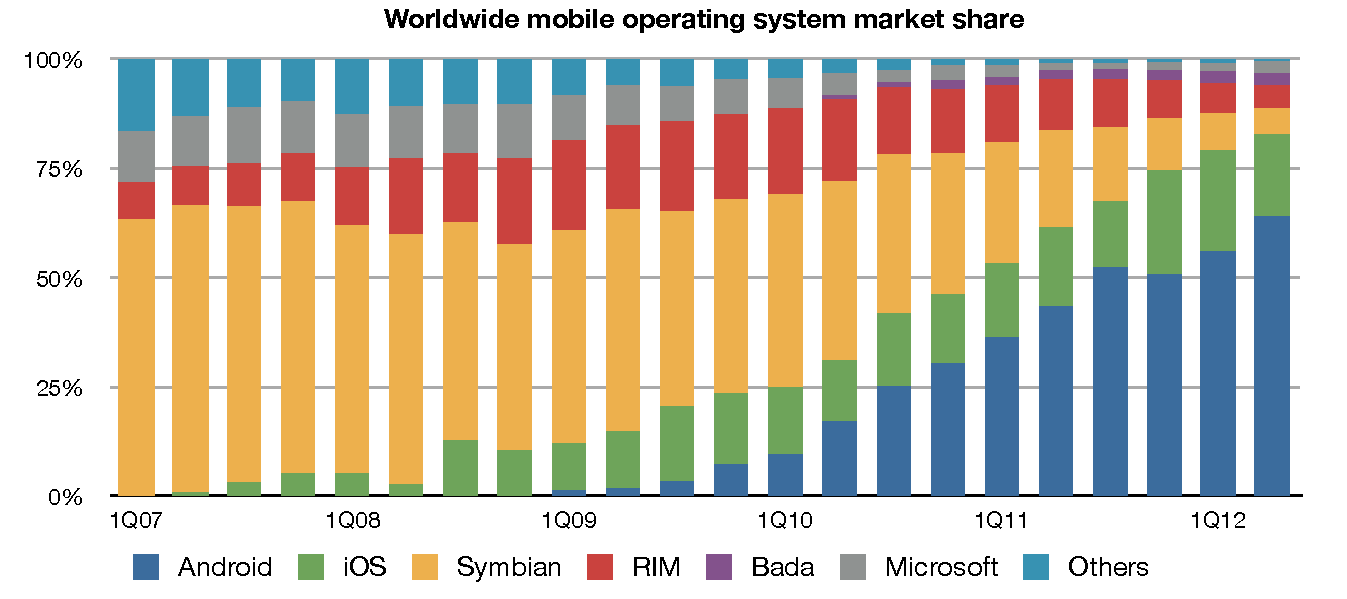
\includegraphics[width=\textwidth]{figs/smartphone_os.pdf}
        \caption{
            Growth of worldwide smartphone operating system market share. Source: Gartner \citep{Gartner:08Q2,Gartner:08Q3,Gartner:08Q4,Gartner:10Q1,Gartner:10Q2,Gartner:10Q3,Gartner:10Q4,Gartner:11Q1,Gartner:11Q2,Gartner:11Q3,Gartner:11Q4,Gartner:12Q1,Gartner:12Q2}
        	}
        \label{fig:smartphone_os}
    \end{center}
\end{figure}

\npar But more importantly, one can conclude that there is not one major platform. Projections by the IDC show that in 2016, there will be at least three major platforms covering 90\% of the worldwide smartphone market \citep{IDC:phone}. 

\npar A similar scenario is playing in the tablet industry. According to other studies by both Gartner \citep{Gartner:11tab,Gartner:12tab} and IDC \citep{IDC:tablet}, tablets will continue to gain popularity and sales will be mainly driven by iPads and Android tablets (see \fref{fig:tablet}).

\begin{figure}[h!]
    \begin{center}
        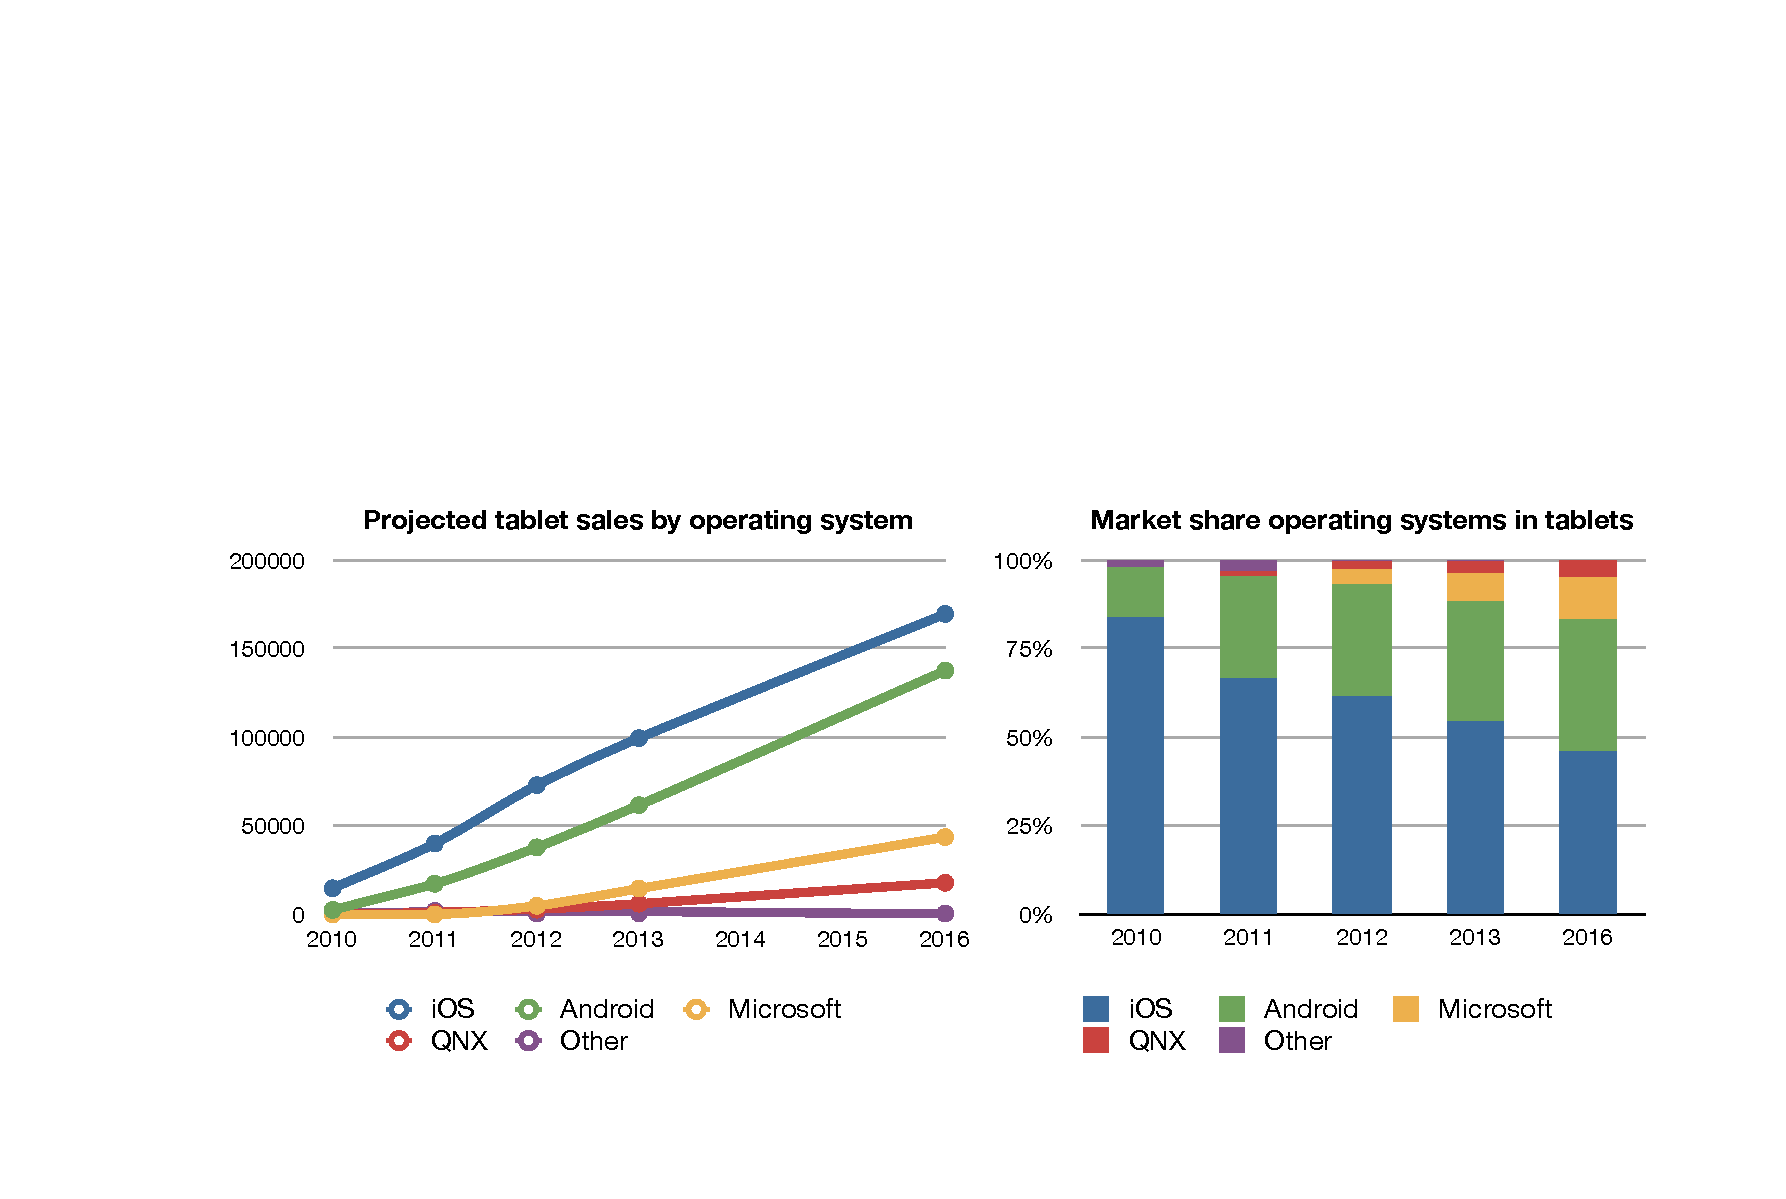
\includegraphics[width=\textwidth]{figs/tablet.pdf}
        \caption{
            Growth of worldwide smartphone sales and smartphone penetration. Source: Gartner \citep{Gartner:11tab,Gartner:12tab}
        }
        \label{fig:tablet}
    \end{center}
\end{figure}

\npar Even though both companies do not agree on which platform will be the biggest by 2016, they both predict there will be at least three major platforms; iOS, Android and Windows. 

% TODO: summary?

\section{The problem of fragmentation}

\npar The competition among mobile device manufacturers has led to fragmentation on many levels. For consumers, fragmentation is usually a good thing. The more different devices there are, the easier it is for a consumer to pick one that fits his needs. For developers on the other hand, fragmentation is usually considered bad. Developers have to develop and test their applications on multiple devices to be able to guarantee the desired experience. This is expensive and time consuming.

\npar From \fref{fig:smartphone_os} and \fref{fig:tablet} it is already clear that the market is divided by operating system or platform but even within these platforms, fragmentation is multi-dimensional \citep{Kindel}.

\npar In general, there are fewer fragmentation problems with Apple's iOS because it is a closed platform. Android, however, is an open source platform and vendors are allowed to tailor it for their devices. As a result, there are hundreds of Android based devices but also hundreds of Android flavours.

\npar Maintenance of such Android flavours is expensive and for this reason, manufacturers do not often provide updates for their devices. This has led to noticeable runtime fragmentation among Android based devices (see \fref{fig:runtime_fragmentation}). Compared to iOS, this is a serious issue.

\begin{figure}[h!]
    \begin{center}
        \label{fig:runtime_fragmentation}
        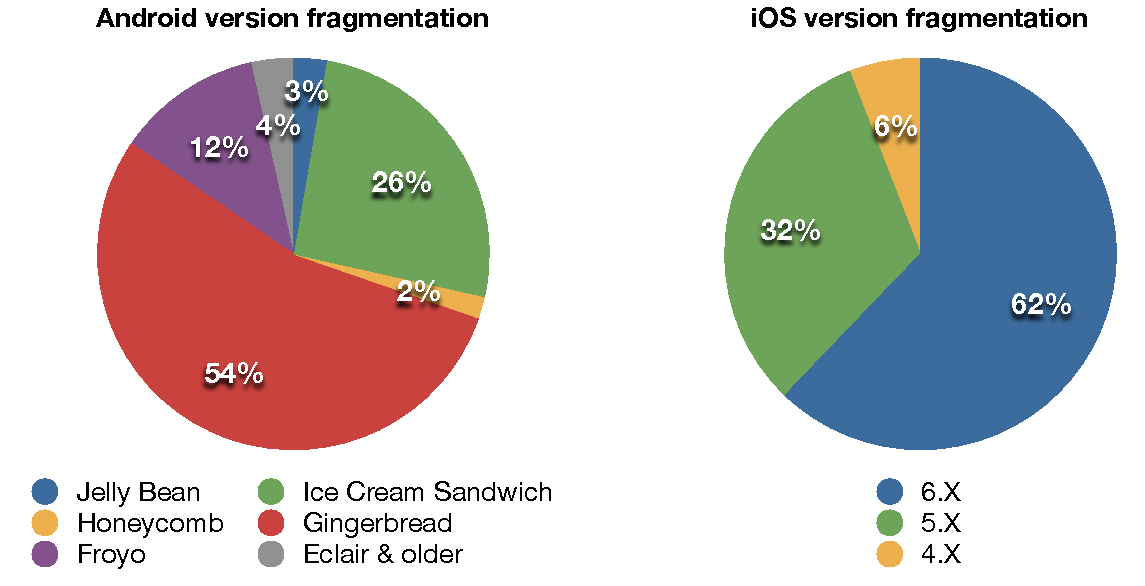
\includegraphics[width=0.8\textwidth]{figs/os_distribution.pdf}
        \caption{
            Runtime fragmentation for Android (data collected by Google during a 14-day period ending on November 1, 2012) \citep{android_distribution} and iOS (based on the statistics of developer David Smith) \citep{ios_distribution}.
        }
    \end{center}
\end{figure}

\npar Fragmentation on the device axis is unavoidable but, again, fragmentation among Android based devices is worse than among iDevices. The most relevant items on this axis are the different hardware specifications and screen resolution.

\npar 

\section{Strategies for cross platform development}

\npar There are already a number of paradigms for cross platform mobile application development \citep{Friese}. This section presents an overview of the available strategies by comparing different aspects: performance, look and feel, platform access, programming languages, development cost and distribution.

\subsection{Native App}

\npar A native app is an application that is specifically designed to run on a particular platform. It is the default approach to develop applications for mobile devices. \fref{fig:native} shows an illustration of the overall architecture of such an app. 

\begin{figure}[h!]
    \begin{center}
        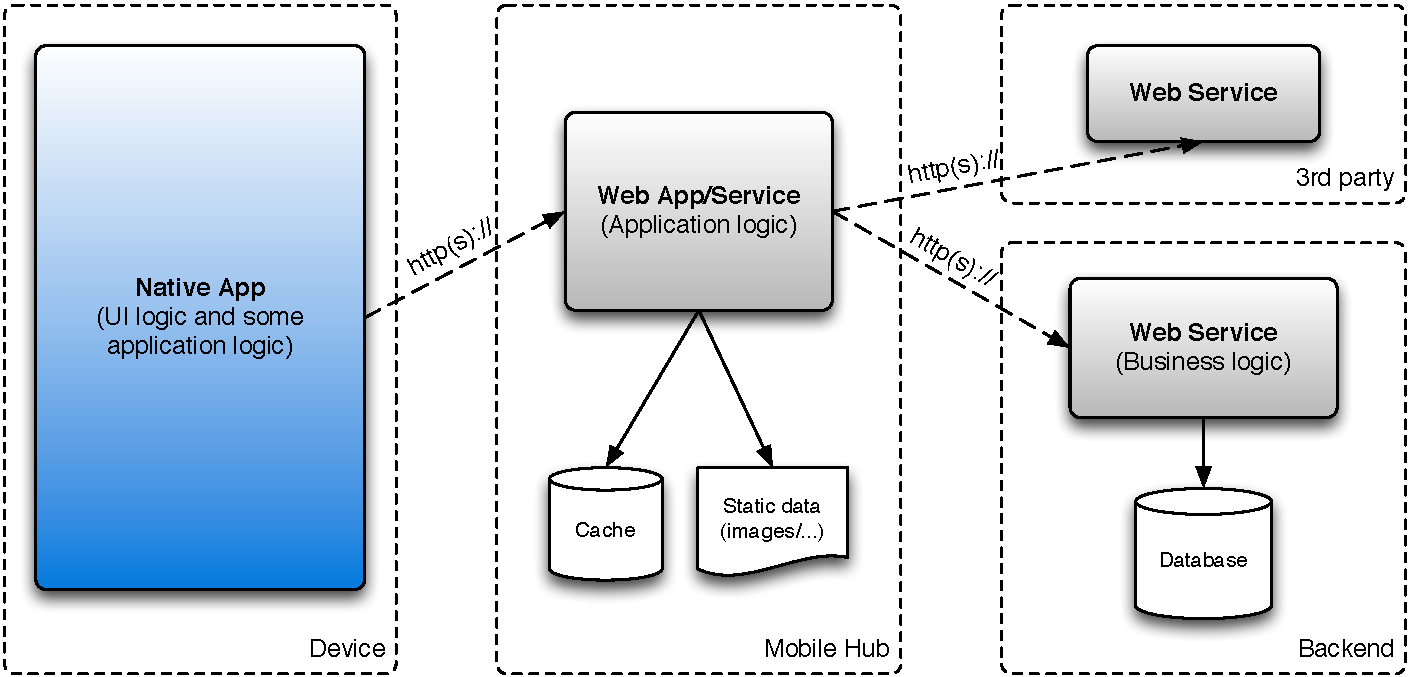
\includegraphics[width=\textwidth]{figs/native.pdf}
        \caption{
            Overall architecture of a native app. 
        }
        \label{fig:native}
    \end{center}
\end{figure}

\npar Native apps are developed with the supplied SDK. Developers will need to get acquainted with the programming language used by said SDK but in return they will get full access to the platform and its features. As a result, the best performance can be obtained with this kind of app.

\npar For the user interface, developers can use lots of interface elements such that they can present a familiar look and feel to the end user. 

\npar Native apps can be easily distributed through an online marketplace like for instance the App Store or Google Play. 

\npar Because native apps are designed to run on one platform only, this development strategy is not very well suited for cross platform development. If an application should run on multiple platforms, it has to be developed for each platform separately. 

% TODO: talk about mobile hub

\subsection{Web App}

\npar Web apps are websites that are optimized for mobile browsers. Since every platform comes with a browser, this is the easiest way to get an application running on all platforms. An overview of the overall architecture for this kind of app is given in \fref{fig:web}.

\begin{figure}[h!]
    \begin{center}
        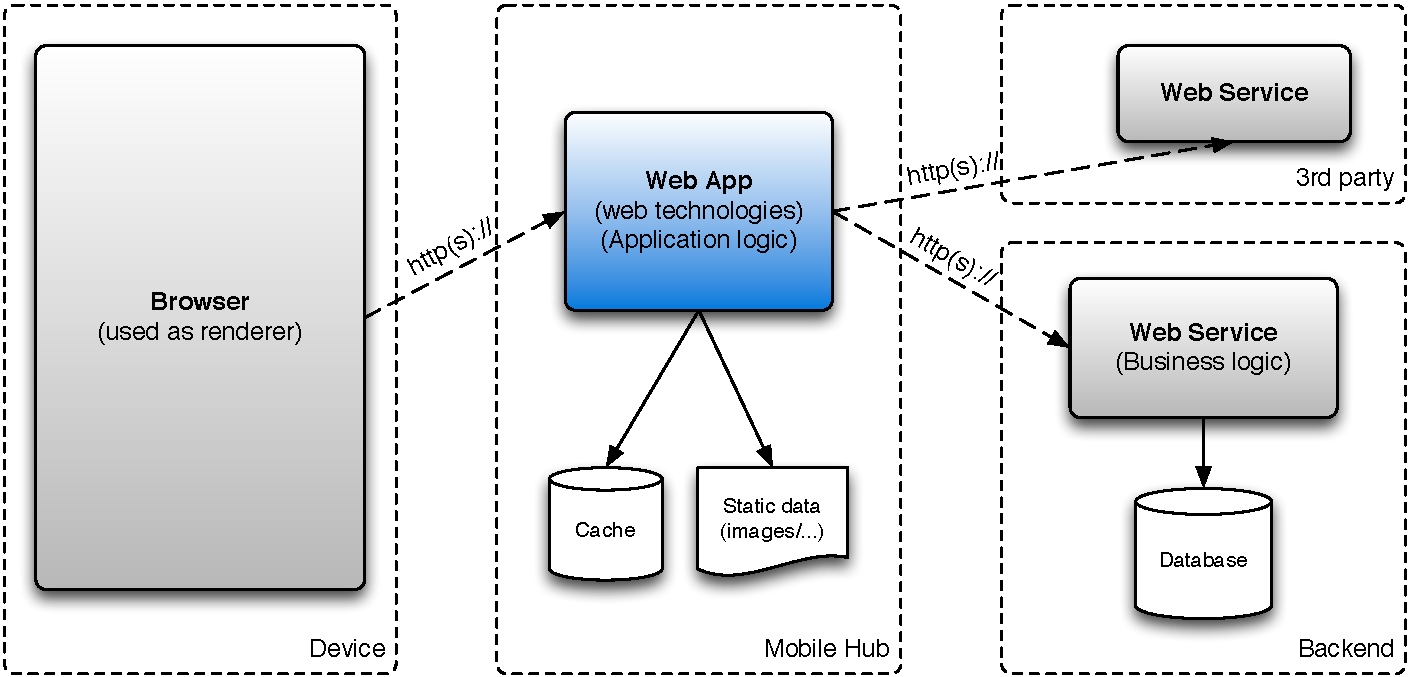
\includegraphics[width=\textwidth]{figs/web.pdf}
        \caption{
            Overall architecture of a web app.
        }
        \label{fig:web}
    \end{center}
\end{figure}

\npar Web apps are not nearly as powerful as native apps. First of all, the application is not stored on the device. Web apps require an active internet connection which cannot always be guaranteed. Second, they are built with web technologies like HTML, CSS and JavaScript, which have to be interpreted by the browser at runtime. Third, web apps cannot access the system which means they cannot make use of the many unique features of a mobile device. 

\npar With HTML5, web apps can get more powerful. They will be able to access device features, like the camera and other sensors \citep{MobileHTML5}. They will not even require an active internet connection because they can be cached on the device. However, HTML5 is still a draft and a lot of mobile browsers lack proper HTML5 support.

\npar From a user interface perspective, web apps can be a problem as well. % TODO: complete paragraph

\npar Web apps are distributed easily: the only requirement is a valid URL. Web apps cannot be installed on the device though, but there are workarounds using Web Clips on iOS \citep{Safari:webclips} and bookmarks on Android. 

\subsection{Hybrid App}

\npar Hybrid applications are the logical next step, combining native apps and web apps. The actual application is a web site, embedded in a web view, part of a native wrapper. An overview of the overall architecture is shown in \fref{fig:hybrid}. 

\begin{figure}[h!]
    \begin{center}
        %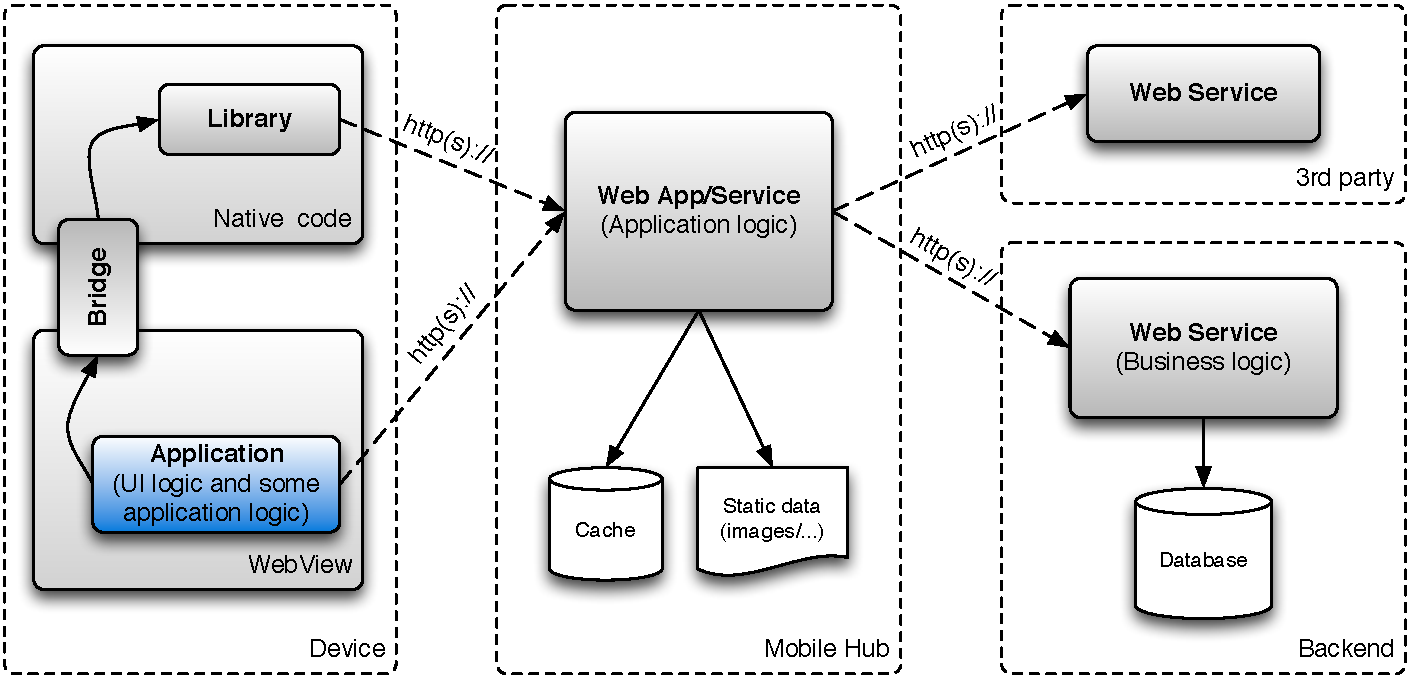
\includegraphics[width=\textwidth]{figs/hybrid.pdf}
        \caption{
            Overall architecture of a hybrid app.
        }
        \label{fig:hybrid}
    \end{center}
\end{figure}

\npar 

\subsection{Interpreted App}

\npar In an interpreted application, instructions are translated to native instructions at runtime.

\begin{figure}[h!]
    \begin{center}
        %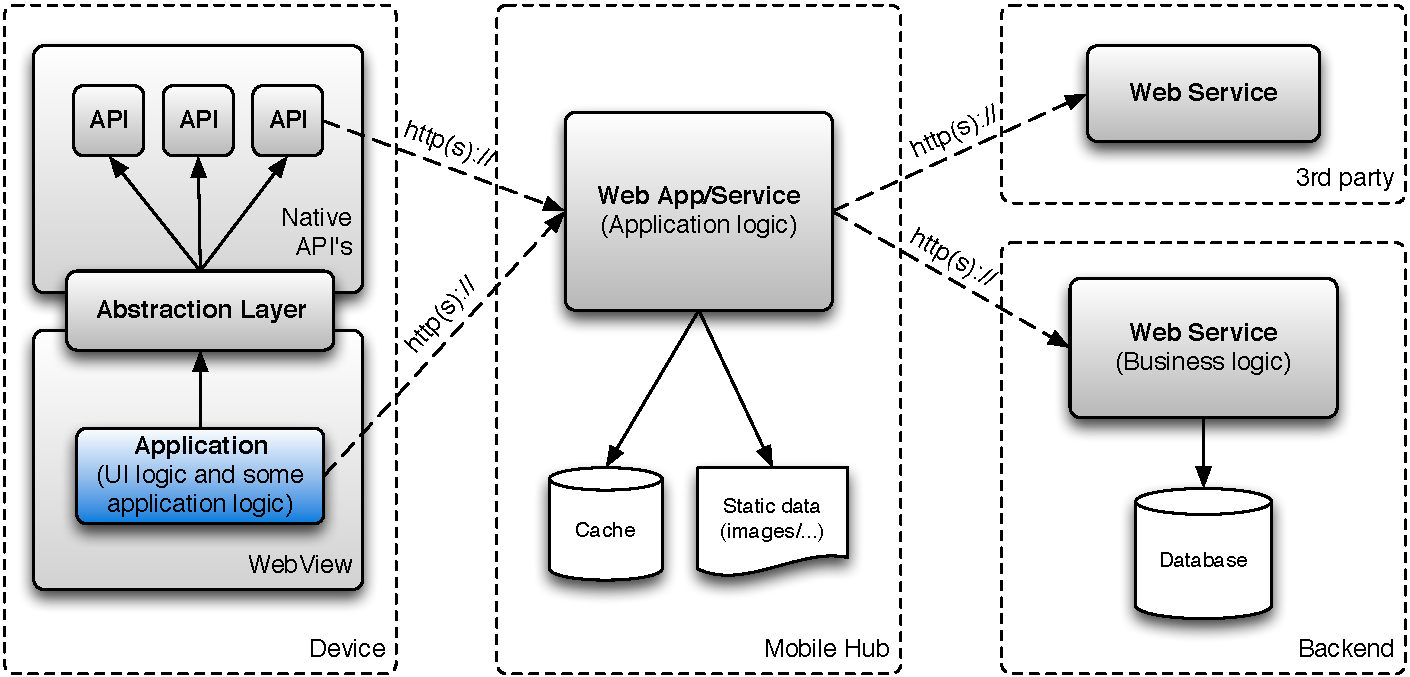
\includegraphics[]{figs/interpreted.pdf}
        \caption{
            Application architecture of an interpreted app, based on \citep{Friese}
        }
        \label{fig:interpreted}
    \end{center}
\end{figure}

\subsection{Cross Compiling}

\npar Instead of translating instructions at runtime, one can translate instructions at compile time. The process is called cross compiling and the result is a truly native app. Performance is similar to native apps but 

\begin{figure}[h!]
    \begin{center}
        %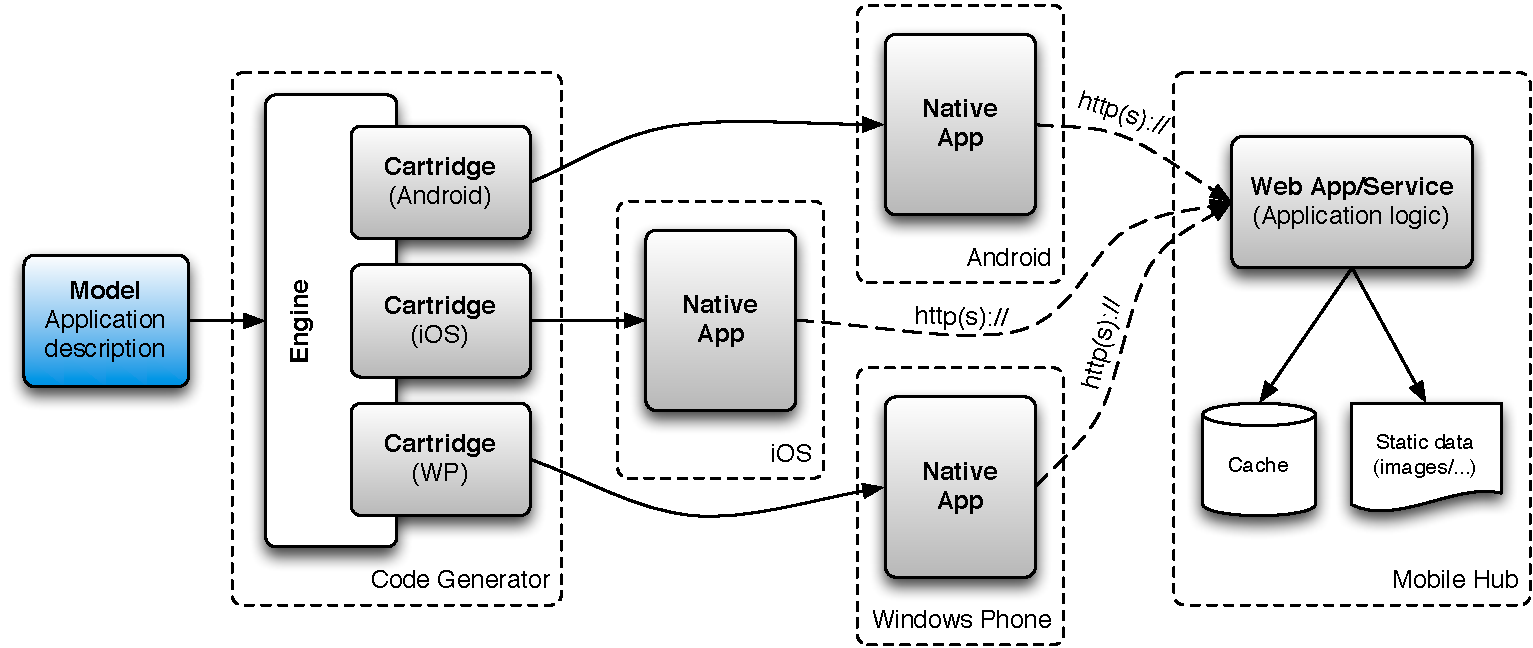
\includegraphics[]{figs/crosscompiled.pdf}
        \caption{
            Architecture used to create cross compiled apps, based on \citep{Friese}
        }
        \label{fig:crosscompiled}
    \end{center}
\end{figure}

\subsection{Summary}

\begin{table}[h!]
    \begin{center}
        \begin{tabular}{l|c|c|c|c|c}
                         & Native App & Web App & Hybrid App & Interpreted App & Cross Compiling\\\hline
            Performance  &            &         &            &                 &                \\
            Look \& Feel &            &         &            &                 &                \\
            Distribution &            &         &            &                 &                \\
            
        \end{tabular}
		\caption{
			Summary of cross platform mobile application development strategies
		}
		\label{tab:architectures}
    \end{center}
\end{table}

\npar

\section{Reflection}

\section{Conclusion}